\documentclass{article}
\usepackage{graphicx}
\usepackage{float}
\title{Graphical Analysis of Heart Disease Dataset}

\begin{document}
	\maketitle
	
	\begin{figure}[H]
		\centering
		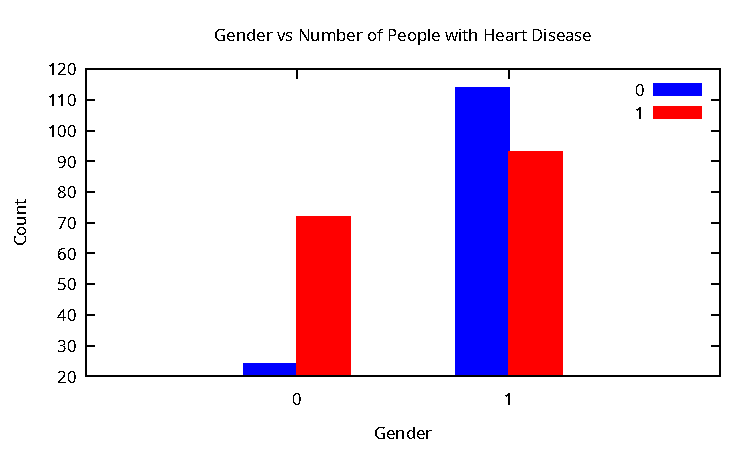
\includegraphics[scale=0.7]{gender_vs_disease.pdf}
		\caption{Distribution of Heart Disease Cases by Gender}
		\label{fig:gender_disease_distribution}
	\end{figure}
	
	\begin{figure}[H]
		\centering
		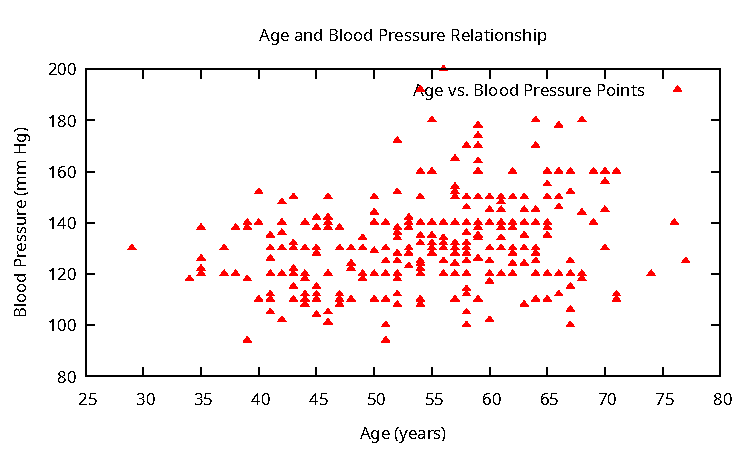
\includegraphics[scale=0.7]{age_bp_relation.pdf}
		\caption{Age and Resting Blood Pressure Relationship}
		\label{fig:age_vs_bp}
	\end{figure}
	
	\begin{figure}[H]
		\centering
		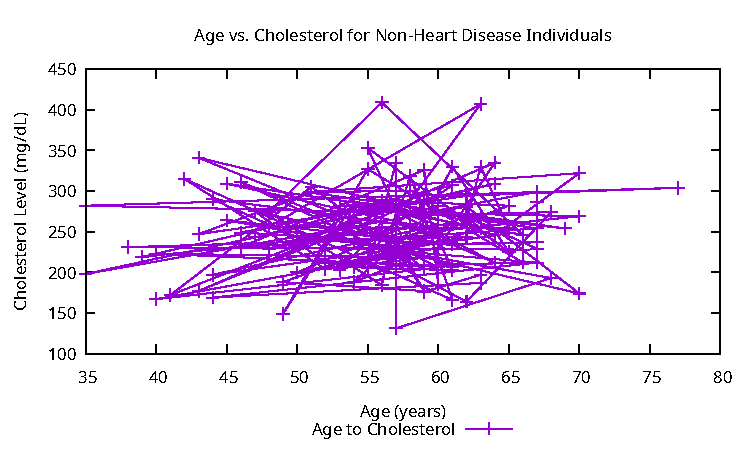
\includegraphics[scale=0.7]{no_heart_chol_chart.pdf}
		\caption{Age vs. Cholesterol Levels in Individuals without Heart Disease}
		\label{fig:age_chol_no_disease}
	\end{figure}
	
	\begin{figure}[H]
		\centering
		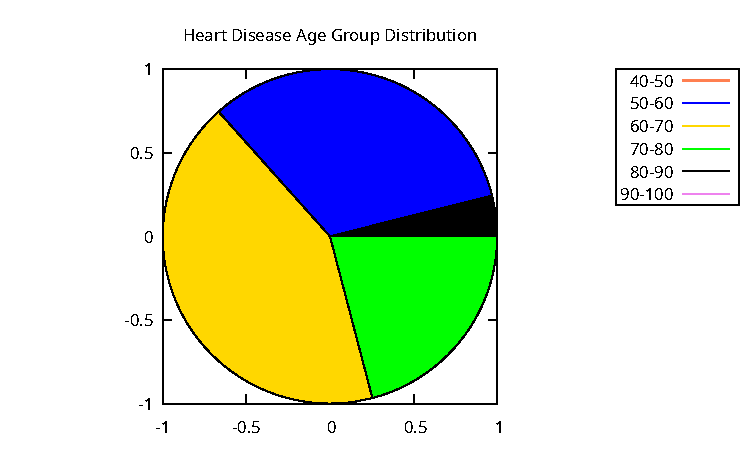
\includegraphics[scale=0.7]{age_distribution_pie.pdf}
		\caption{Age Group Proportion of Heart Disease Cases (Pie Chart)}
		\label{fig:age_disease_pie}
	\end{figure}
	
\end{document}
